\documentclass[11pt,a4paper]{ctexart}
\usepackage[margin=1in]{geometry}
\usepackage{amsmath,amssymb,mathtools}
\usepackage{booktabs}
\usepackage{graphicx}
\usepackage{hyperref}
\usepackage{caption}
\usepackage{subcaption}
\usepackage{placeins}
\usepackage{float}

\title{自动驾驶交通标志识别中的神经网络安全验证：基于抽象解释与线性松弛的可证鲁棒性分析}
\author{}
\date{}

\newcommand{\R}{\mathbb{R}}
\newcommand{\B}{\mathcal{B}}
\newcommand{\relu}{\operatorname{ReLU}}
\renewcommand{\abstractname}{摘要}
\renewcommand{\refname}{参考文献}
\raggedbottom
\setlength{\textfloatsep}{8pt plus 1pt minus 2pt}
\setlength{\floatsep}{8pt plus 1pt minus 2pt}
\setlength{\intextsep}{8pt plus 1pt minus 2pt}
\makeatletter
\setlength{\@fptop}{0pt}
\setlength{\@fpsep}{8pt plus 1pt minus 2pt}
\setlength{\@fpbot}{0pt plus 1fil}
\makeatother

\begin{document}
\maketitle

\begin{abstract}
交通标志识别是自动驾驶视觉感知链路中的安全关键环节。仅凭经验攻击测试无法给出可靠的安全保证，因此本文研究输入扰动约束下 ReLU 分类网络的可证鲁棒性验证问题。我们将问题形式化为局部最坏情况 margin 最优化，并比较区间界传播、抽象解释中的线性松弛，以及引入 0-1 变量的 MILP 精化三类方法。实验基于 GTSRB 的三类交通标志子集进行，结果表明，当扰动半径从 $\varepsilon=0.002$ 增大到 $\varepsilon=0.01$ 时，IBP 的认证率由 $0.9$ 下降到 $0$，而 LP 与 MILP 仍分别保持 $0.5$ 和 $0.6$。这说明更紧的松弛和局部精化对于安全关键感知任务中的形式化验证具有直接价值。
\end{abstract}

\section{引言}
自动驾驶系统必须在复杂道路环境中稳定识别交通标志。若分类器在微小像素扰动下输出错误类别，后续控制决策便可能失效。与仅依赖攻击样本的经验评估不同，可证鲁棒性希望给出形式化保证：对任意满足扰动约束的输入，模型输出的正确类别优势保持为正。GTSRB 数据集为交通标志识别提供了标准评测基准 \cite{stallkamp2011gtsrb}，而 DeepPoly、IBP、MILP 等方法则构成了当前可证鲁棒性研究的重要技术主线 \cite{singh2019deeppoly,singh2019boosting,gowal2018ibp,tjeng2017mip}。

本文围绕此问题展开：给定交通标志图像 $x_0$、真实标签 $y$ 和扰动半径 $\varepsilon$，如何证明
\[
\arg\max_k f_k(x)=y,\qquad \forall x\in \{x:\|x-x_0\|_\infty\le \varepsilon\}.
\]
我们选择 ReLU 网络作为分析对象，因为它既是视觉模型的常见构件，也具有分段线性结构，适合用多元统计、非线性优化和整数规划的方法进行验证。

本文的主要工作是把交通标志识别中的安全问题形式化为局部鲁棒性验证问题，并在同一个小型网络和同一组扰动半径下比较 IBP、LP 松弛与 MILP 精化。本文的目的是展示一个数学事实：同样的分类模型在经验准确率相同的情况下，可能因为验证外包络的松紧程度不同而得到完全不同的安全结论。

\section{问题形式化}
设分类器 $f:\R^d\to \R^K$ 为一个带 ReLU 激活的前馈网络。输入图像 $x_0\in[0,1]^d$，真实标签为 $y$。考虑 $L_\infty$ 扰动球
\[
\B_\infty(x_0,\varepsilon)=\{x\in[0,1]^d:\|x-x_0\|_\infty\le \varepsilon\}.
\]
鲁棒性验证问题可写为
\[
\forall x\in \B_\infty(x_0,\varepsilon),\quad f_y(x)\ge f_j(x),\ \forall j\neq y.
\]
定义 margin
\[
m_j(x)=f_y(x)-f_j(x),
\]
则只要对每个 $j\neq y$ 有 $\inf_{x\in\B_\infty(x_0,\varepsilon)} m_j(x)>0$，就可认证该样本鲁棒。

进一步地，可以把验证问题写成一组最优化子问题：
\[
\gamma_j(x_0,\varepsilon)=\min_{x\in\B_\infty(x_0,\varepsilon)} \bigl(f_y(x)-f_j(x)\bigr),\qquad j\neq y.
\]
若对所有 $j\neq y$ 都有 $\gamma_j(x_0,\varepsilon)>0$，则样本 $x_0$ 在半径 $\varepsilon$ 下通过认证。这个写法的好处在于，它把“安全”变成了一个可以计算的下界问题：我们并不需要穷举扰动后的所有输入，只需要对每个竞争类别求一个最坏情况下界。

该问题虽然由分段线性网络诱导，但整体上并不是简单凸优化问题。输入 $x$ 是连续变量，隐藏层预激活与激活值也是连续变量，而每个不稳定 ReLU 的开闭状态对应离散模式选择。

从安全解释角度看，$\gamma_j$ 不只是一个优化目标，而是一个可审计的安全证据。当 $\gamma_j>0$ 时，它表示在整个扰动球内正确类别 $y$ 的 logit 都严格大于竞争类别 $j$；当某个 $\gamma_j\le 0$ 时，验证器无法排除类别 $j$ 在局部邻域内超过真实类别的可能性。这里需要区分“认证失败”和“真实存在攻击”：前者可能来自模型确实脆弱，也可能来自松弛过松。本文后续同时报告 IBP、LP 和 MILP，正是为了区分这两种原因。

自动驾驶中的交通标志识别错误不是普通分类错误，而可能影响车辆减速、让行或限速决策。经验测试只能说明有限测试样本上没有观察到错误，而局部鲁棒性验证试图证明一个连续输入集合上的性质。把有限样本测试提升为连续集合上的保证，是可证安全方法区别于常规机器学习评测的关键。

\section{数学背景与直观解释}
\subsection{ ReLU 难验证的原因}
对某个预激活 $z$，$\relu(z)=\max(0,z)$。若区间边界满足 $l\ge 0$ 或 $u\le 0$，该神经元状态是稳定的；若 $l<0<u$，则该神经元是否激活不确定，这正是验证的主要难点。可以把它理解成一个开关：输入扰动范围内，开关状态是否固定，决定了后续层的几何形状是否可控。

\subsection{三种包络}
本文比较的三种方法可以理解为三种不同精度的外包络。区间传播只记录每层激活的上下界，速度快，但把不同维度之间的相关性全部丢掉，因此容易得到过松的安全下界。线性松弛或抽象解释方法保留变量之间的线性约束，把真实可达集包在一个多面体内，通常比轴对齐区间更紧。MILP 精化则进一步对关键不稳定 ReLU 引入二元变量，显式刻画开关状态，从而减少松弛误差。这个“从粗到细”的思想与 Wong 和 Kolter 的凸外包络方法 \cite{wong2018convex} 以及 DeepPoly 的抽象域传播 \cite{singh2019deeppoly} 一脉相承。

\begin{figure}[htbp]
  \centering
  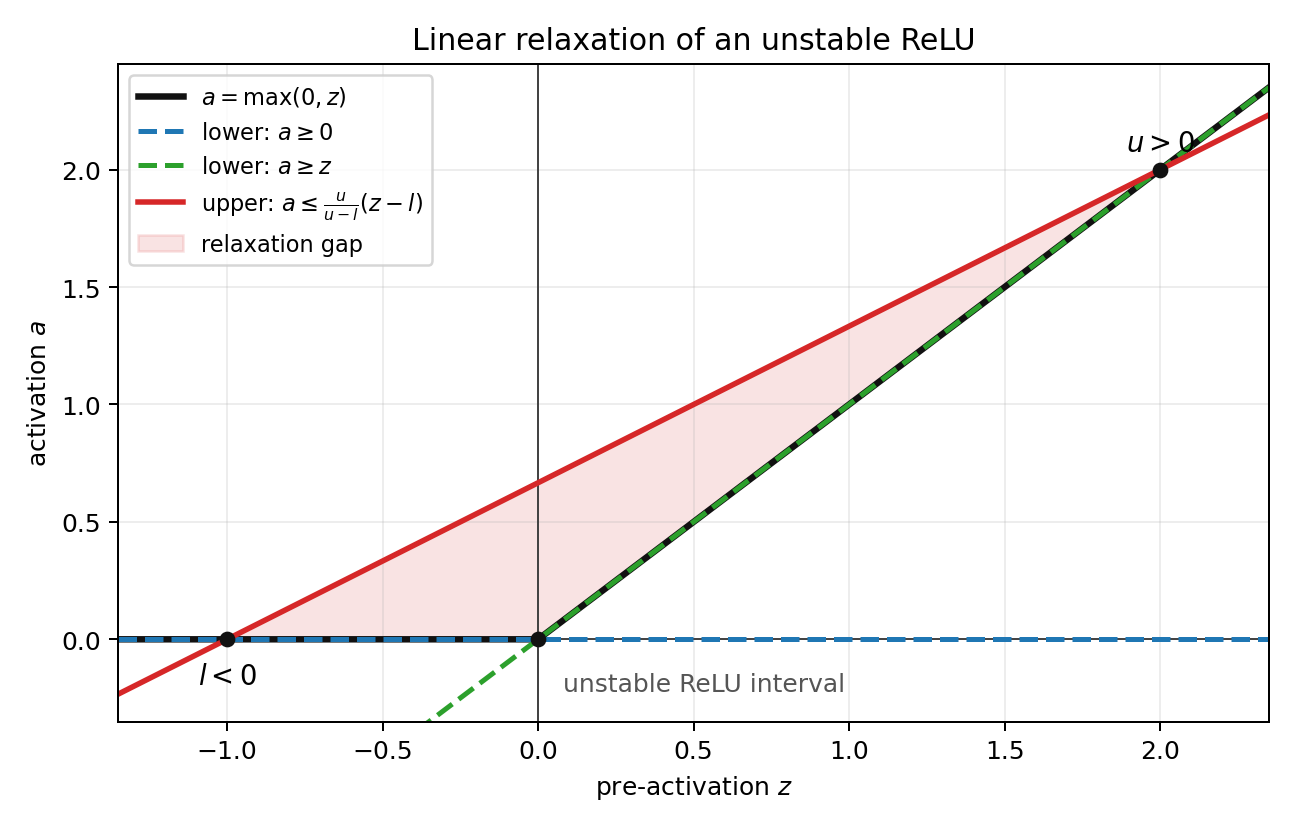
\includegraphics[width=0.78\linewidth]{outputs/relu_relaxation.png}
  \caption{ReLU 在不稳定区间 $l<0<u$ 上的线性松弛示意。黑色折线是真实 ReLU，蓝色和绿色虚线给出两个下界约束，红色直线给出上界约束，阴影区域表示松弛带来的 gap。}
  \label{fig:relu}
\end{figure}

\begin{figure}[htbp]
  \centering
  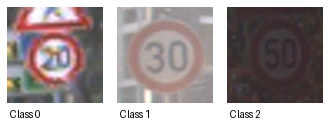
\includegraphics[width=0.72\linewidth]{outputs/gtsrb_samples.png}
  \caption{GTSRB 三类交通标志样本示意图。}
  \label{fig:samples}
\end{figure}
\FloatBarrier

\subsection{相关工作与本文定位}
交通标志识别本身是自动驾驶感知中的经典问题，GTSRB 为该任务提供了较成熟的数据基准 \cite{stallkamp2011gtsrb}。在可证鲁棒性方向上，相关工作大致可以分为三类。第一类是凸松弛与线性外包络方法，例如 Wong 与 Kolter 提出的 convex outer adversarial polytope \cite{wong2018convex}；第二类是基于抽象解释的传播方法，例如 DeepPoly \cite{singh2019deeppoly}；第三类是基于混合整数规划的精确或半精确验证方法 \cite{tjeng2017mip,singh2019boosting}。另外，IBP 与 CROWN-IBP 代表了训练可证鲁棒模型的一条重要路线 \cite{gowal2018ibp,zhang2020crownibp}。



\section{方法分析}
\subsection{区间界传播}
对仿射层 $z=Wx+b$，若 $x\in[l,u]$，则
\[
z_{\min}=W^+l+W^-u+b,\qquad z_{\max}=W^+u+W^-l+b,
\]
其中 $W^+=\max(W,0)$，$W^-=\min(W,0)$。随后对 ReLU 逐坐标截断即可。

IBP 的优点是实现简单、速度快，而且每一层只需要维护两个向量。它的弱点也来自同一个设计：当两个神经元在真实网络中强相关时，区间传播仍把它们当作可以独立取上下界的变量。层数增加后，这种独立化误差会不断累积，导致最终 margin 下界被严重低估。因此，IBP 更适合做快速筛查，而不是对边界样本给出最终判断。

\subsection{线性松弛}
当 $l<0<u$ 时，可用
\[
a\ge 0,\qquad a\ge z,\qquad a\le \frac{u}{u-l}(z-l)
\]
刻画 ReLU 的凸外包络。对多层网络，将这些局部线性约束串联后，可用线性规划求 margin 下界。若下界仍大于零，则原网络安全。这个松弛之所以有效，是因为它保留了“输入变化如何沿着权重传导”的线性结构，而不是把每一层都独立地粗暴裁剪掉。与 CROWN-IBP 的思想类似，更紧的线性界通常能显著提升认证率 \cite{zhang2020crownibp}。

在本文实现中，LP 验证器显式构造输入变量、每层预激活变量和每层 ReLU 输出变量。输入变量满足 $x_i\in[\max(0,x_{0,i}-\varepsilon),\min(1,x_{0,i}+\varepsilon)]$，仿射层通过等式约束连接，ReLU 层通过图~\ref{fig:relu} 中的三条线性不等式外包。对每个竞争类别 $j$，目标函数设置为最小化 $f_y(x)-f_j(x)$。如果这个线性规划的最优值仍为正，就说明即使在外包络放宽后的更大集合中，竞争类别也无法超过真实类别，因此原始网络在该扰动半径下必然安全。

\subsection{MILP 精化}
对不稳定 ReLU 引入二元变量 $s\in\{0,1\}$，令
\[
a\ge z,\quad a\ge 0,\quad a\le z-l(1-s),\quad a\le us.
\]
这样可将分段线性结构精确编码为 MILP。其优点是精度高，缺点是变量数和求解时间随不稳定神经元数量快速增长。因此，MILP 不适合大规模全量验证，但很适合对边界样本做“最后一道确认”，这正符合安全系统中的分层验证思路。类似的混合整数验证思路已在早期工作中得到系统讨论 \cite{tjeng2017mip,singh2019boosting}。

MILP 与 LP 的差别可以从几何上理解。LP 允许 ReLU 在不稳定区间内取红色上界与真实折线之间的任意点，因此可行域包含了原网络不可能产生的伪激活模式。MILP 用二元变量把“关闭”和“打开”两种模式分开，相当于把这个伪区域切掉。由此得到的下界更接近真实最坏情况，但整数变量会引入分支定界搜索，运行时间也更容易受样本局部几何影响。

\subsection{复杂度与安全含义}
验证问题的核心矛盾是可扩展性与紧致性之间的张力。粗松弛方法容易扩展到更多样本，但可能无法证明边界样本安全；精确或半精确方法能给出更强保证，却需要付出更高计算代价。安全关键系统中的合理做法通常不是只选择一种方法，而是先用便宜方法筛掉明显安全或明显不安全的样本，再把边界样本交给更强的优化器。

从实现角度看，IBP 的代价主要来自逐层上下界传播，近似与网络规模线性相关；LP 松弛在每个样本、每个竞争类别上都需要求解一个线性规划，因此代价显著增加；MILP 则在此基础上再引入整数变量，其最坏情况复杂度增长更快。也正因为如此，MILP 更适合作为局部精化工具，而不是全量主力验证器。。

\section{实现与实验}
\subsection{实验设置}
实验使用 GTSRB 数据集的三类交通标志子集（类别 $0,1,2$），每类最多抽取 $120$ 张训练样本。为保证验证计算可控，所有图像统一转为 $16\times16$ 灰度图，并训练一个单隐层 ReLU MLP，隐藏层宽度设为 $32$。验证阶段选取 $10$ 个测试样本，分别在 $\varepsilon\in\{0.002,0.005,0.01\}$ 下比较 IBP、LP 松弛与 MILP 精化。

在实现层面，本文没有直接调用现成的端到端验证器，而是自行实现了三条核心链路：一是基于区间上下界的 IBP；二是基于 ReLU 线性外包络的 LP 松弛；三是基于整数变量的 MILP 精化。求解器部分使用 \texttt{scipy.optimize.linprog} 与 \texttt{scipy.optimize.milp}，从而保证整条实验链在普通 Python 环境中可复现。

为保证复现链路完整，脚本还保留了 sklearn digits 数据集的 sanity check 模式，但本文正文中的主结果均基于 GTSRB 子集。

数据处理流程保持有意简化。原始交通标志图像尺寸和光照条件并不一致，实验脚本先读取图像与标签，再按类别筛选出三类子集，随后统一缩放为 $16\times16$ 并转换为灰度输入。。

训练和验证被明确分开。模型训练只用于获得一个具有非线性决策边界的小型 ReLU 分类器；验证阶段不再更新参数，而是把已训练网络视为固定函数 $f$，围绕测试样本构造扰动球并求解最坏 margin。这个设置避免把“鲁棒训练”和“鲁棒验证”混在一起，也使实验结论更直接地指向验证器本身的松紧差异。

\subsection{评价指标}
实验主要报告四类指标：clean accuracy、certified accuracy、平均验证时间以及失败案例数量。这里的 clean accuracy 反映模型在原始测试样本上的分类能力；certified accuracy 则只统计那些既被正确分类、又能在给定半径下被形式化认证的样本。两者并不等价：高 clean accuracy 并不必然带来高 certified accuracy，这正是安全验证区别于普通分类评测的地方。

\begin{table}[H]
\centering
\caption{GTSRB 三类子集上的认证结果（$n=10$，clean accuracy = 0.9）。}
\begin{tabular}{ccccc}
\toprule
$\varepsilon$ & IBP & LP 松弛 & MILP & 平均时间(s) \\
\midrule
0.002 & 0.9 & 0.9 & 0.9 & 0.038 \\
0.005 & 0.5 & 0.9 & 0.9 & 0.095 \\
0.010 & 0.0 & 0.5 & 0.6 & 0.280 \\
\bottomrule
\end{tabular}
\label{tab:results}
\end{table}

\begin{table}[H]
\centering
\caption{不同隐藏层宽度下的结果对比（$\varepsilon=0.005$）。}
\begin{tabular}{ccccc}
\toprule
隐藏层宽度 & clean acc & IBP & LP / MILP & 平均时间(s) \\
\midrule
8 & 0.9 & 0.6 & 0.8 & 0.019 \\
16 & 0.8 & 0.6 & 0.7 & 0.024 \\
32 & 0.9 & 0.5 & 0.9 & 0.097 \\
\bottomrule
\end{tabular}
\label{tab:width}
\end{table}

\begin{figure}[H]
  \centering
  \begin{subfigure}{0.49\linewidth}
    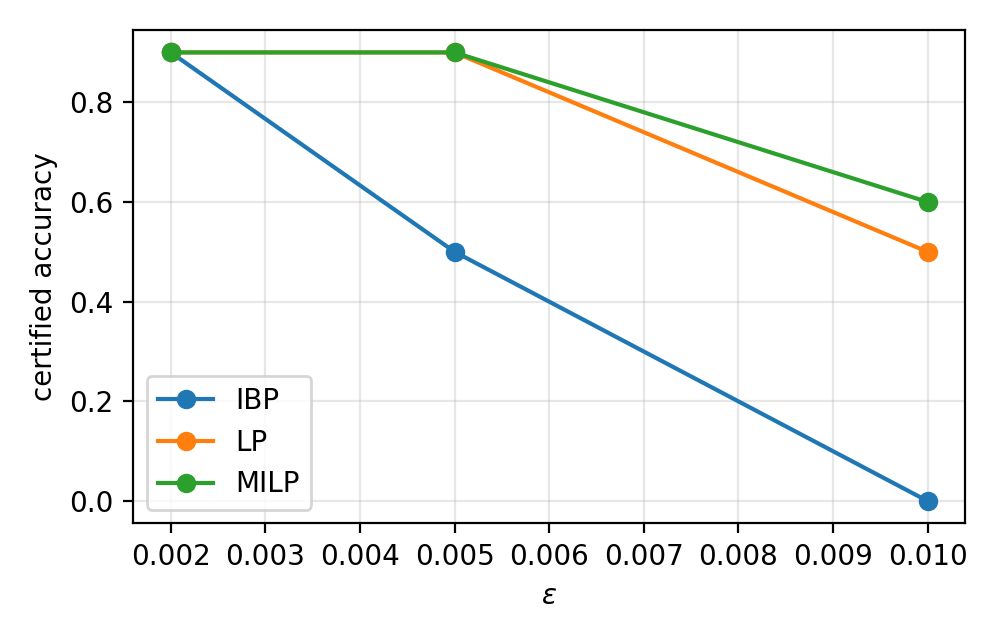
\includegraphics[width=\linewidth]{outputs/certified_accuracy_curve.png}
    \caption{认证率随 $\varepsilon$ 变化。}
  \end{subfigure}
  \hfill
  \begin{subfigure}{0.49\linewidth}
    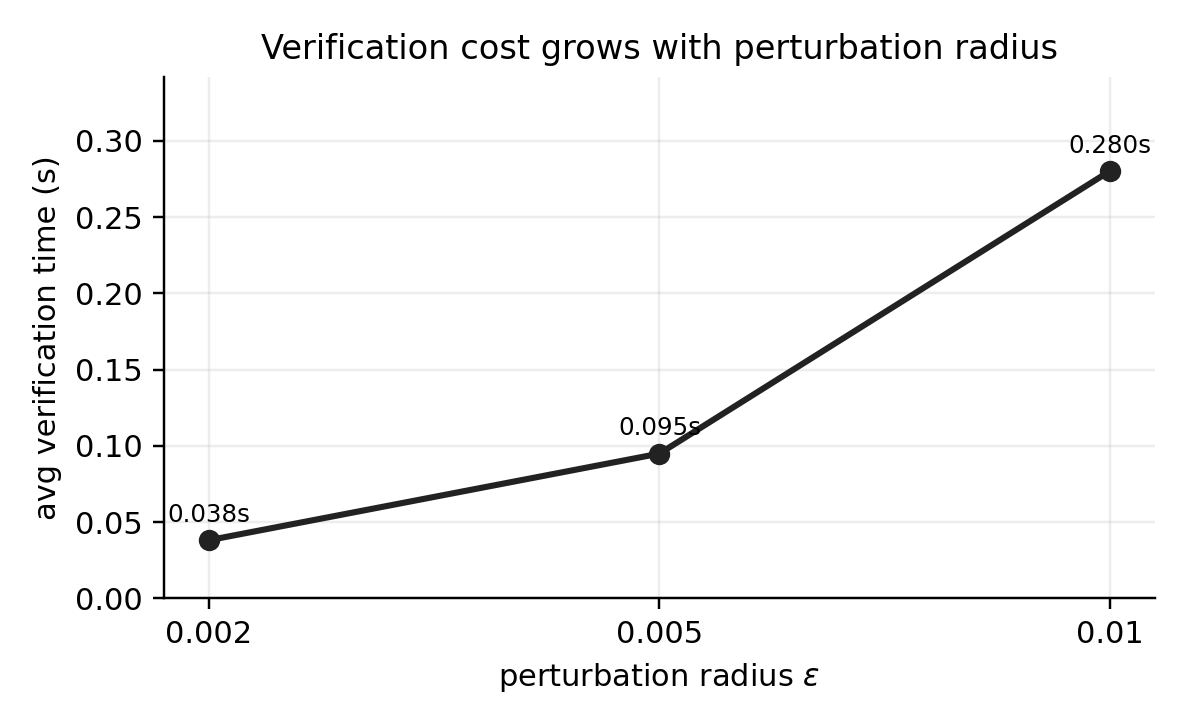
\includegraphics[width=\linewidth]{outputs/epsilon_time_curve.png}
    \caption{平均验证时间随 $\varepsilon$ 变化。}
  \end{subfigure}
  \caption{扰动半径对认证率和验证时间的影响。随着扰动球扩大，更多 ReLU 进入不稳定区间，认证率下降而验证时间上升。}
  \label{fig:eps_results}
\end{figure}

\begin{figure}[H]
  \centering
  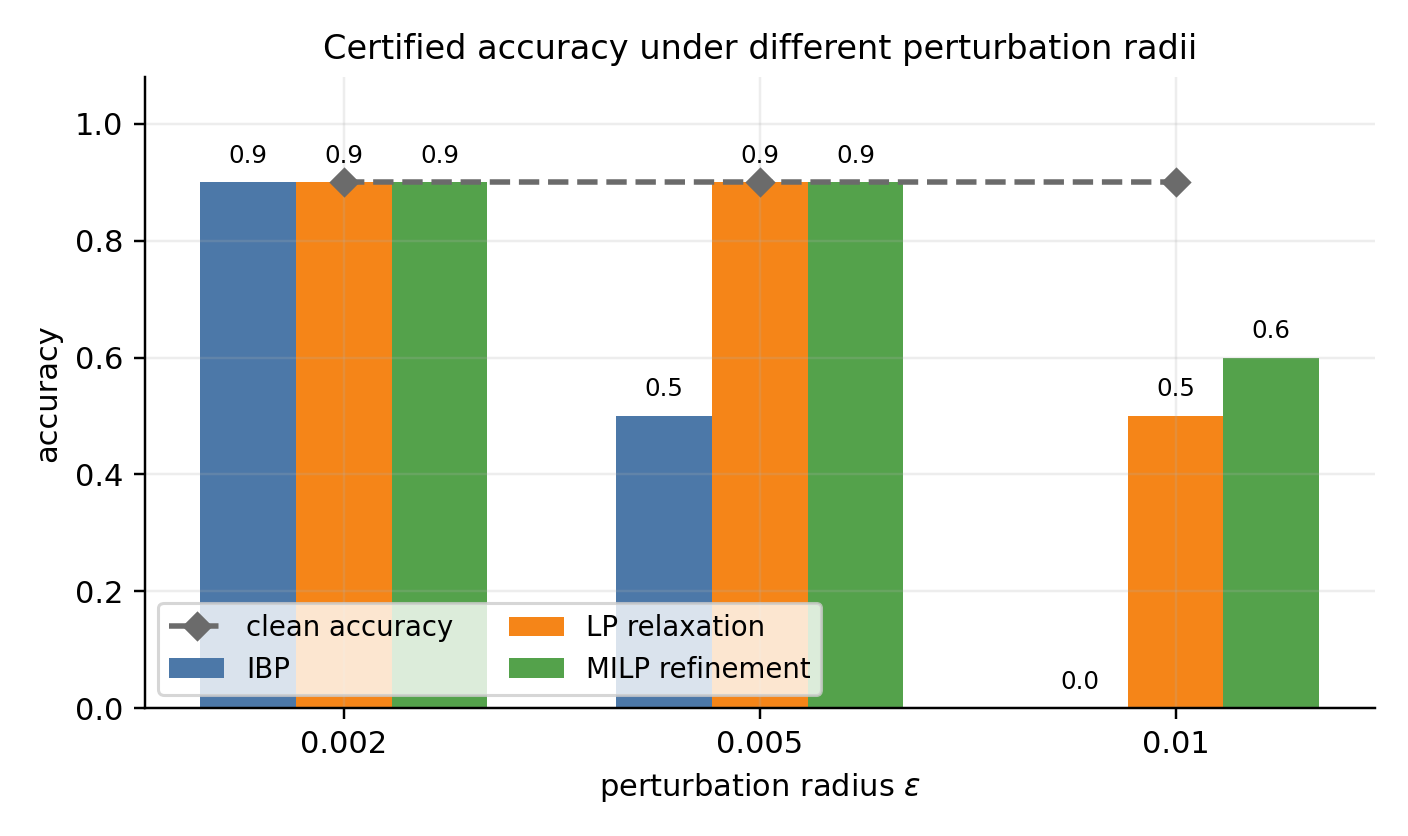
\includegraphics[width=0.76\linewidth]{outputs/certification_bar_by_epsilon.png}
  \caption{不同扰动半径下 clean accuracy 与三种认证方法的 certified accuracy。该图直接对应表~\ref{tab:results}，三组柱分别为 IBP、LP 松弛和 MILP 精化，虚线为 clean accuracy。}
  \label{fig:cert_bar}
\end{figure}

\begin{figure}[H]
  \centering
  \begin{subfigure}{0.49\linewidth}
    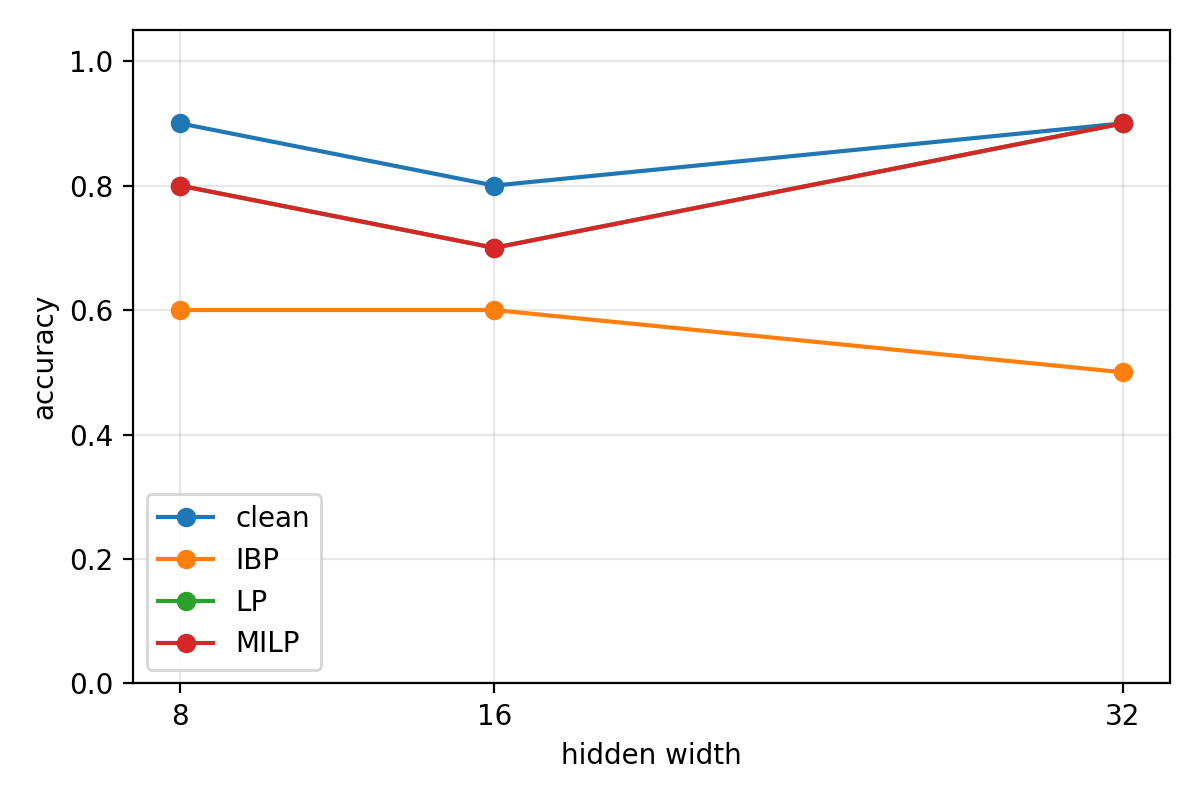
\includegraphics[width=\linewidth]{outputs/width_accuracy_curve.png}
    \caption{宽度与认证率。}
  \end{subfigure}
  \hfill
  \begin{subfigure}{0.49\linewidth}
    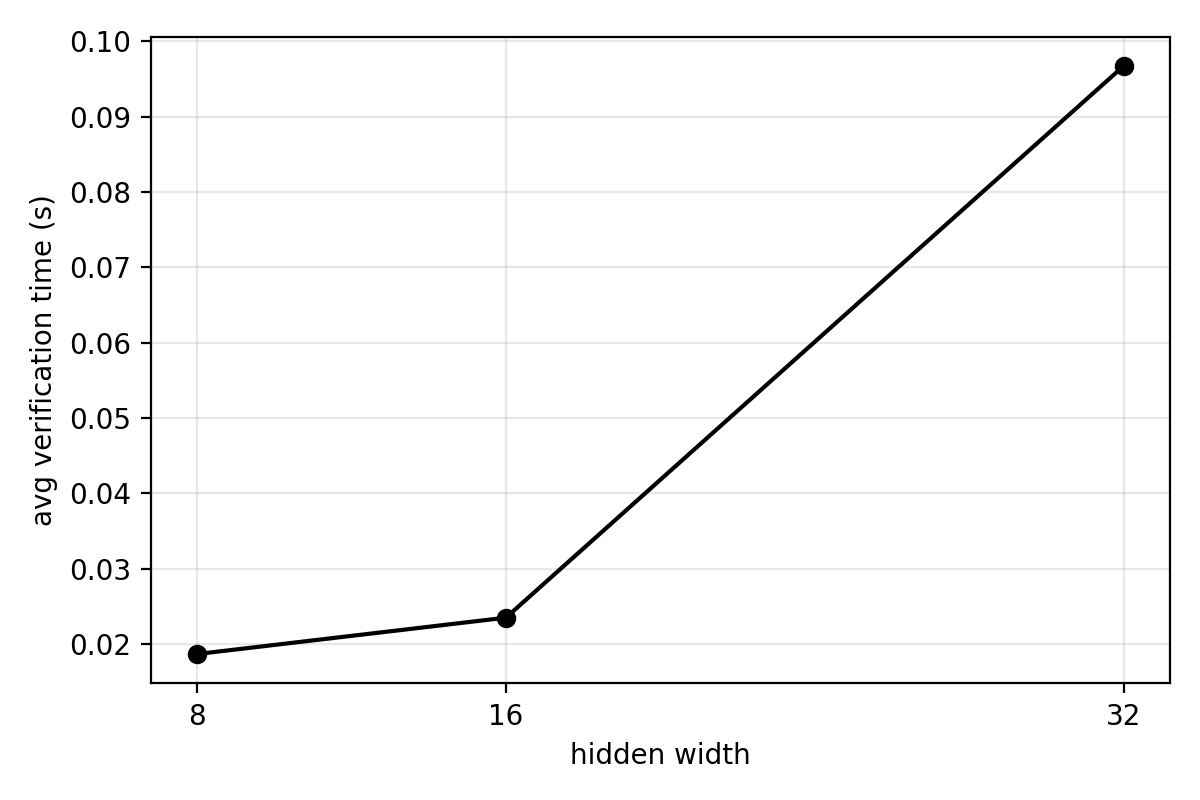
\includegraphics[width=\linewidth]{outputs/width_time_curve.png}
    \caption{宽度与验证时间。}
  \end{subfigure}
  \caption{隐藏层宽度对分类准确率、认证率和验证时间的影响。}
  \label{fig:width_results}
\end{figure}

\begin{figure}[H]
  \centering
  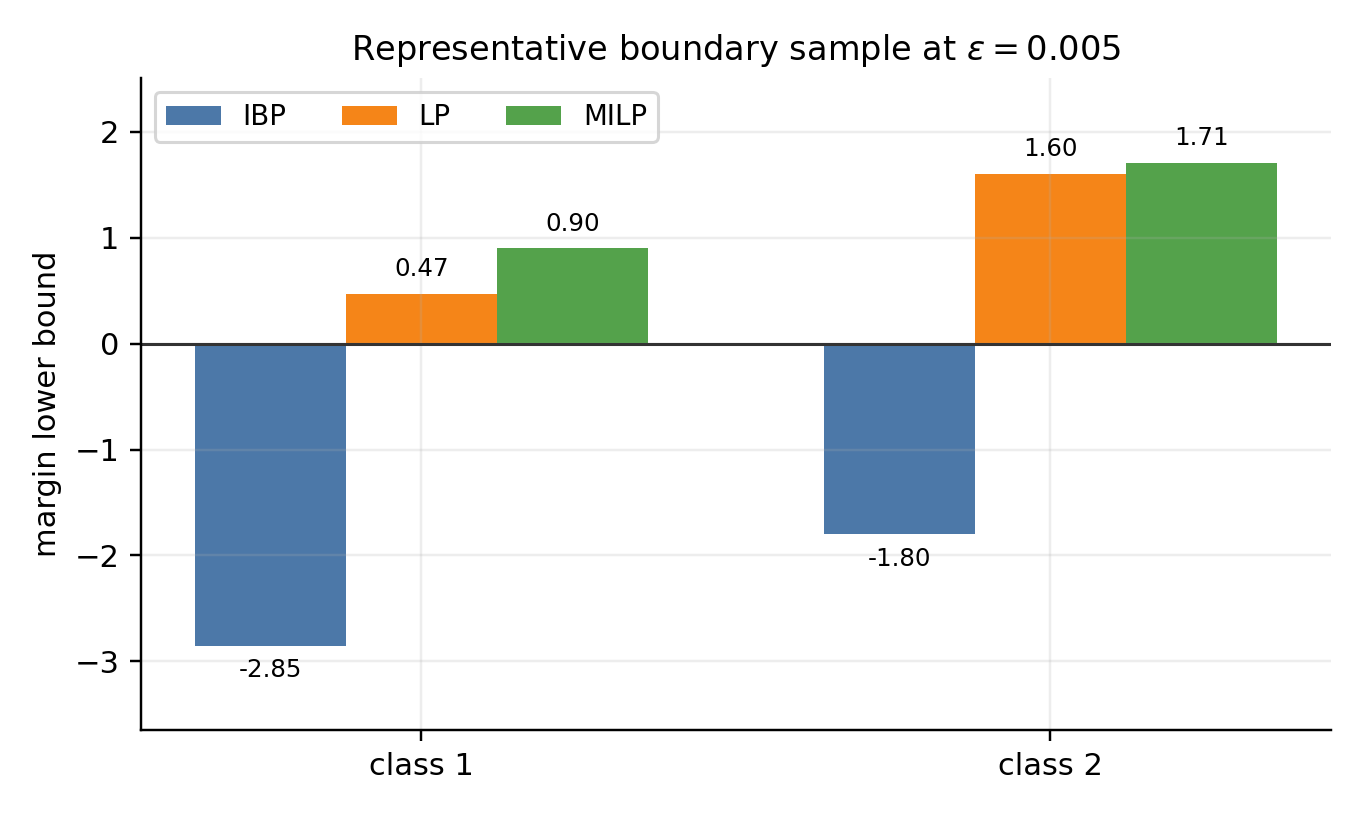
\includegraphics[width=0.76\linewidth]{outputs/sample_margin_comparison.png}
  \caption{代表性边界样本上三种方法的 margin 下界比较。IBP 给出负下界，而 LP 和 MILP 均给出正下界。}
  \label{fig:margin_compare}
\end{figure}

\begin{figure}[H]
  \centering
  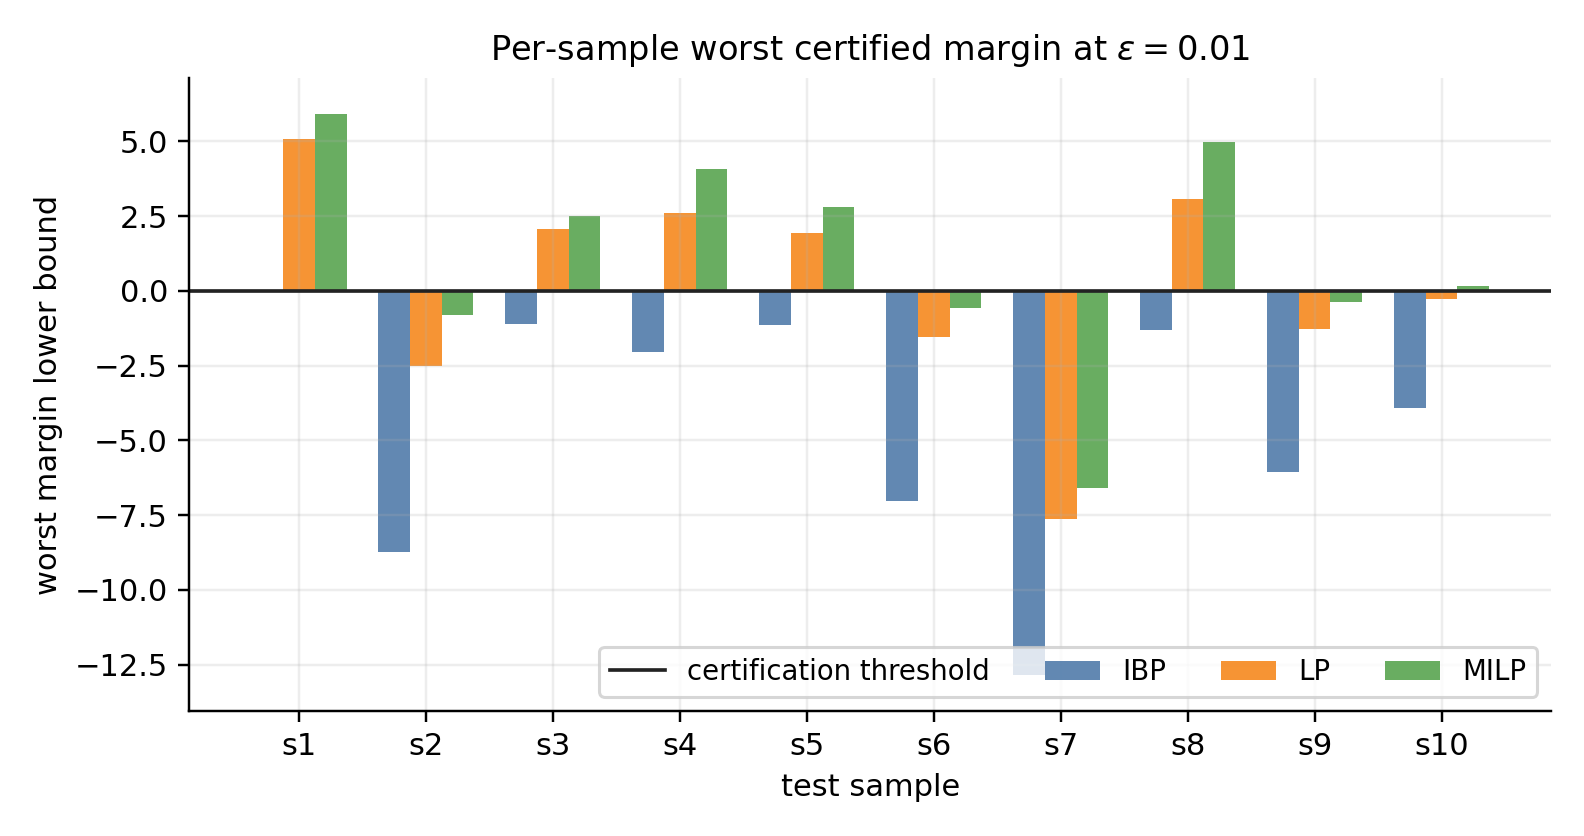
\includegraphics[width=0.90\linewidth]{outputs/per_sample_worst_margin_bar.png}
  \caption{逐样本最坏 margin 下界。黑色水平线是认证阈值 $0$；柱子高于 0 表示该方法能证明该样本在当前扰动半径下安全。该图对应的认证数量为 IBP $0/10$、LP $5/10$、MILP $6/10$。}
  \label{fig:sample_results}
\end{figure}

\subsection{结果解读与失败案例}
表~\ref{tab:results}、图~\ref{fig:eps_results} 和图~\ref{fig:cert_bar} 给出的结论一致：扰动半径越大，认证越困难。当 $\varepsilon=0.002$ 时，三种方法都能认证 $90\%$ 的测试样本；当 $\varepsilon=0.005$ 时，IBP 降到 $50\%$，但 LP 与 MILP 仍保持 $90\%$；当 $\varepsilon=0.01$ 时，IBP 无法认证任何样本，而 LP 和 MILP 分别还能认证 $50\%$ 和 $60\%$。

从 \texttt{outputs/hidden32/rows.jsonl} 中可以看到，边界样本上最典型的现象是：IBP 给出的某个竞争类别 margin 下界为负，而 LP 或 MILP 可以把该下界重新拉回正区间。例如某一类 $0$ 的样本在 $\varepsilon=0.005$ 下，IBP 对类别 $1$ 的 margin 下界为 $-2.85$，但 LP 和 MILP 分别将其提高到 $0.47$ 与 $0.90$；对类别 $2$，IBP 下界为 $-1.80$，LP 与 MILP 分别提高到 $1.60$ 与 $1.71$。图~\ref{fig:margin_compare} 直接画出了这一记录，因此该样本不是“真实攻击已经找到”，而是区间传播给出的下界过于保守。

与此同时，也存在 LP 与 MILP 都无法认证的样本。例如在 $\varepsilon=0.01$ 下，某一类 $0$ 样本的 MILP 下界仍为负值，说明即使进行精化，该样本在给定扰动球内也缺乏足够的安全边际。这类失败案例提醒我们：认证失败并不总是算法问题，有时反映的是模型本身在局部邻域内确实不够稳健。
\FloatBarrier

\section{个人见解}
首先，表~\ref{tab:results} 和图~\ref{fig:cert_bar} 说明，clean accuracy 在三个扰动半径下保持 $0.9$，但 certified accuracy 随 $\varepsilon$ 增大明显下降。这正说明普通分类准确率不能替代安全认证指标：模型在原始图像上分类正确，并不意味着它在连续扰动球内也保持同一预测。

其次，图~\ref{fig:eps_results} 展示了认证率下降和验证时间上升这两个现象的同步发生。$\varepsilon$ 从 $0.002$ 增大到 $0.01$ 时，平均验证时间从 $0.038$ 秒增加到 $0.280$ 秒。原因是扰动球扩大后，隐藏层中更多 ReLU 跨过 $0$，从稳定神经元变成不稳定神经元，LP 和 MILP 都需要处理更多有效约束或分支状态。

从图~\ref{fig:margin_compare} 可以更细致地看到松弛紧致性的影响。对于这个边界样本，IBP 在两个竞争类别上都给出负下界，因此无法认证；LP 和 MILP 则都给出正下界，因此可以认证。MILP 对类别 $1$ 的下界从 LP 的 $0.47$ 进一步提高到 $0.90$，说明整数精化确实能缩小松弛 gap；但对类别 $2$，LP 的 $1.60$ 与 MILP 的 $1.71$ 差距很小，说明并不是每个竞争类别都值得付出 MILP 代价。

宽度实验提供了第二层观察。表~\ref{tab:width} 和图~\ref{fig:width_results} 表明，网络宽度增大并不单调提升 clean accuracy，但会显著增加验证时间。具体地，隐藏层宽度从 8 增加到 32 时，平均验证时间从约 0.019 秒增加到约 0.097 秒，而 LP/MILP 的认证率收益并非线性增长。这说明在安全关键场景中，模型容量和可验证性之间存在明显张力：更大的模型可能拥有更强的拟合能力，但也会带来更多不稳定 ReLU，从而提高验证代价。

图~\ref{fig:sample_results} 则从逐样本角度补充了这一结论。图中直接把每个样本的最坏 margin 下界画出来，黑线以上表示通过认证，黑线以下表示失败。整体上，LP 和 MILP 都把更多样本的下界推到了 0 以上，对应认证数量分别为 $5/10$ 和 $6/10$，而 IBP 在 $\varepsilon=0.01$ 下为 $0/10$。


从实验结果看，验证方法的“保守性”本身也是安全系统需要管理的风险。过松的验证器会把一部分真实安全的样本判为无法认证，造成假阴性；过于昂贵的精确验证器又可能无法覆盖足够多的样本，造成工程部署困难。因此，在实际自动驾驶系统中，更现实的方案是分层部署：IBP 用于快速筛查，LP 用于常规认证，MILP 用于边界样本和高风险类别的重点复核。本文的小规模实验虽然不能直接替代工业系统评估，但清楚展示了这种分层思想的数学原因。

\subsection{局限性与未来工作}
本文仍有几个明显局限。第一，实验模型采用的是小型单隐层 MLP，这降低了工程复杂度，但也限制了结论的外推范围。第二，正文只使用了 GTSRB 的三类子集和 10 个测试样本做认证演示，而不是工业级大规模验证。第三，当前采用的是灰度缩放输入，这在一定程度上简化了视觉结构。

未来工作可以沿三个方向展开。其一，换用卷积结构并比较卷积网络与 MLP 在可验证性上的差别；其二，引入更多类别和更大的测试集，以观察统计结论是否稳定；其三，研究分支定界、神经元优先级策略以及更紧的凸松弛，从而进一步缩小 LP 与 MILP 间的 gap。

\subsection{小结}
本文从交通标志识别这一安全关键任务出发，将神经网络局部鲁棒性验证形式化为一个可计算的最坏情况优化问题，并比较了抽象解释、线性松弛与 MILP 精化三类方法。GTSRB 子集实验表明，随着扰动半径增大，粗松弛方法的认证率会显著退化，而更紧的 LP 松弛与 MILP 精化能够维持更高的安全保证。

后续若继续扩展，可进一步研究卷积结构、更多类别、以及分支定界对认证效率的影响。



\bibliographystyle{plain}
\bibliography{references}

\clearpage
\appendix
\section{实验说明}
本文实验脚本默认支持 GTSRB 与 sklearn 的 digits 两种数据源。正文主结果基于 GTSRB 三类交通标志子集；digits 模式仅用于方法连通性验证。脚本已实现三个方法：IBP、LP 松弛和 MILP 精化，并输出每个样本的 margin 下界与 summary JSON。

输出文件包括三个 JSON 类记录文件和多张实验图像。\texttt{summary.json} 记录单组实验的总体结果，\texttt{rows.jsonl} 记录逐样本下界与认证状态，\texttt{sweep\_summary.json} 记录不同 $\varepsilon$ 下的 sweep 结果。图像文件对应正文中的认证率曲线、样本示意图、宽度对比图和代表性样本下界图。这些输出一方面支撑正文中的图表，另一方面也保证了结果的可追溯性：任何表格中的数值都可以回溯到具体的 JSON 或逐样本记录。


\end{document}
